\documentclass[10pt]{article}
\usepackage[margin=0.78in]{geometry}
\usepackage{amsmath,amssymb,bm}
\usepackage{booktabs}
\usepackage{graphicx}
\usepackage{enumitem}
\usepackage[hidelinks]{hyperref}
\usepackage{caption}
\captionsetup{font=small,labelfont=bf,skip=4pt}
\setlist{nosep,leftmargin=1.4em}
\setlength{\parskip}{2pt}
\setlength{\abovedisplayskip}{4pt}\setlength{\belowdisplayskip}{4pt}
\newcommand{\Tr}{\mathrm{Tr}}
\newcommand{\bPsi}{\bar\Psi}
\newcommand{\bQ}{\bar Q}
\title{\vspace{-1.6cm}\Large\textbf{Bootstrapping Matrix SYK Models}\vspace{-4pt}}
\author{}
\date{}

\begin{document}
\maketitle
\vspace{-1.1cm}
\begin{center}\begin{minipage}{0.94\textwidth}\small
\textbf{Abstract.} ``Matrix SYK'' models are purely fermionic $U(N)$ matrix quantum mechanics with a cubic supercharge, $Q=\sum C_{abc}\Tr\Psi^a\Psi^b\Psi^c$, $H=\{Q,\bQ\}$. The three-flavour version proposed by Chen is the simplest candidate for a matrix model whose BPS sector is \emph{fortuitous} and \emph{R-charge concentrated}, the two properties that in $\mathcal N=2$ SYK produce a super-Schwarzian low-energy description and black-hole-like BPS microstate counting. Its Hilbert space is finite ($2^{3N^2}$), so full exact diagonalisation (ED) is limited to $N=2$ --- at $N=3$ only the few-particle sectors remain accessible by a sector-restricted (``few-body'') ED, the half-filling sectors having dimension up to $2\times10^7$ --- and its ground states in the interesting sectors have no classical large-$N$ saddle. We are developing the quantum-mechanical matrix bootstrap as the tool for $N>2$. We report: a sector-resolved finite-$N$ bootstrap that is exact for the single-matrix model at $N\le4$ and for the three-matrix model at $N=2$ in every sector tested; an exact finite-$N$ \emph{trace} formulation whose cost is independent of $N$, which proves $E_0(k;N)=16N^3-(15+38k)N$ for the $k\le N-1$ sectors at any $N$ and gives the first rigorous bound in an interacting sector at $N=3$; an exact refined Witten index that reproduces the Turiaci--Witten $\cos(\pi k/3)$ BPS profile and exhibits $e^{cN^2}$ multiplicities per irrep; and a ``BPS-exclusion'' bootstrap that rules out BPS states sector by sector in seconds at any $N$, currently reaching half-way to the BPS window. The combination of index and exclusion is a concrete route to establishing R-charge concentration at $N=3,4$.
\end{minipage}\end{center}

\section{Introduction}
\textbf{The models.} Let $\Psi^a_{ij}$ ($a=1..p$, $i,j=1..N$) be complex fermionic $N\times N$ matrices, $\{\Psi^a_{ij},\bPsi^b_{kl}\}=\delta^{ab}\delta_{il}\delta_{jk}$, with $U(N)$ acting by conjugation. The models are defined by a nilpotent cubic supercharge and its Hamiltonian,
\begin{equation}
Q=\sum_{a,b,c}C_{abc}\,\Tr\!\big[\Psi^a\Psi^b\Psi^c\big],\qquad H=\{Q,\bQ\}\ \ge0,\qquad [N_\Psi,Q]=3Q,\quad N_\Psi=\Tr\Psi^a\bPsi^a .
\end{equation}
For $p=1$, $Q=\Tr\Psi^3$ is Chen's single-matrix model~\cite{Chen:2025fortuity}, which is exactly solvable: $H=3N(N^2-1)-9\hat C_2$ is a function of the gauge Casimir, and the BPS ($E=0$) states fill a window of $N+1$ consecutive R-charges $N_\Psi\in[\tfrac{N(N-1)}2,\tfrac{N(N+1)}2]$. For $p=3$ with Chen's couplings $C_{abc}$ (the cyclic symmetrisation of the indicator function of $a\le b\le c$) the Casimir structure is broken: we derived the exact single-trace form of $H$ (nine-term formula with a $\Tr\Psi^c\Tr\bPsi^d$ piece that couples the trace modes) and showed it is \emph{not} a function of Casimirs. This ``three-matrix model'' is the target.

\textbf{Why it is interesting.} In $\mathcal N=2$ SYK~\cite{Fu:2016SUSYSYK} the BPS states are concentrated in an $O(1)$ window of R-charges around half filling, with counts following $\cos(\pi k/3)$; this is the hallmark of the $\mathcal N=2$ super-Schwarzian~\cite{Turiaci:2023N2JT} and, in the fortuity picture of Chang--Lin~\cite{Chang:2024covering,Chang:2024fortuitySYK}, of a BPS sector made of black-hole-like ``fortuitous'' states with $e^{cN^2}$ multiplicities that are not captured by any large-$N$ saddle. The single-matrix model fails this test (window of width $N+1$, all states in one enormous irrep with $O(1)$ multiplicity). The three-matrix model at $N=2$ has 972 BPS states in exactly three sectors, $N_\Psi\in\{5,6,7\}$, with counts $243{:}486{:}243$ --- the $1{:}2{:}1$ SYK pattern. Nobody knows what happens for $N\ge3$.

\textbf{Research questions.} (Q1) Does the three-matrix model exhibit R-charge concentration for $N\ge3$ --- an $O(1)$ window, $\cos(\pi k/3)$ counts, $e^{cN^2}$ multiplicities per irrep? (Q2) Is it chaotic (Altland--Zirnbauer statistics of the singular values of $Q$ between adjacent sectors)? (Q3) Is three the ``magic number'' --- the minimal flavour structure that breaks the Casimir shortcut, introduces genuine R-charge dynamics and chaos? (Q4) What are the energies of the near-BPS sectors and how do they scale with $N$ (the super-Schwarzian predicts gaps $\propto q^2$)?

\textbf{Distinctives, and why the bootstrap.} The models have no bosons: the Hilbert space is the $2^{pN^2}$-dimensional Fock space, every operator algebra truncates, and everything is finite-dimensional linear algebra in principle --- but $2^{27}$ at $N=3$ already puts the full spectrum out of reach (only sectors with $\lesssim10^5$ states, i.e.\ $k\le4$ particles, can still be diagonalised exactly), and $2^{48}$ at $N=4$ ends ED for good. There is no classical large-$N$ saddle for the states of interest (fortuitous states are maximal-Casimir, far from singlets), so the standard planar bootstrap with factorisation is blind to precisely the physics we want. This is the setting in which a \emph{rigorous, finite-$N$} bootstrap --- lower bounds on sector ground energies, and infeasibility certificates for BPS states --- is the natural tool, and, we argue, a promising one.

\section{Methodology}
\textbf{Sector-resolved bootstrap at finite $N$.} The object is the ground energy $E_0(k)$ of the charge sector $N_\Psi=k$. We optimise over linear functionals $\phi(O)=\Tr[\rho_k P_kOP_k]$ with $\rho_k$ Hermitian (not assumed positive) on the $k$-block,
\begin{equation}
\boxed{\;\min_{\rho_k=\rho_k^\dagger}\ \phi(H)\quad\text{s.t.}\quad
\phi(\mathbf 1)=1,\ \
\big[\phi(\Tr w_a^\dagger w_b)\big]\succeq0,\ \
\big[\phi((\Tr w_a)^\dagger\Tr w_b)\big]\succeq0,\ \
\phi([H,X])=0,\ \ \phi((N_\Psi-k)X)=0\;}
\label{eq:sdp}
\end{equation}
where $w$ runs over \emph{open} (adjoint-valued) words in the letters $\Psi^a,\bPsi^a$ up to length $L$ (the ``level''), the two positivity conditions are the adjoint and singlet channels of the Gram matrix of the states $w_{ij}|\psi\rangle$, and $X$ runs over all operators appearing in the cones. Every constraint is satisfied by the exact sector ground state, so the minimum is a rigorous lower bound on $E_0(k)$ that improves monotonically with $L$; the dual is a sum-of-squares certificate $H-E\succeq0$ on the sector, the analogue of the CFT bootstrap functional. Two ingredients turned out to be decisive: (i) the sector projection (charged operators have $\phi=0$ and $[H,X]$ acts within the block), and (ii) restricting to $SU(N)_{\rm gauge}\times\mathbb Z_3$-invariant $\rho_k$, which costs nothing (group averaging) and legitimises Cho et al.'s singlet/adjoint split of the Gram matrix~\cite{Cho:2024thermal}, $\phi(\Tr w_a^\dagger w_b)-\tfrac1N\phi(\Tr w_a^\dagger\Tr w_b)\succeq0$. Implemented with an isotypic decomposition of the block ($\rho_k=\oplus_R\sigma_R\otimes\mathbf 1$, $D=\sum_Rm_R^2$ parameters instead of $d_k^2$), the SDP has at most $D=90$ unknowns at $N=2$, $k=2$ and $666$ at $k=3$. The cost is nevertheless set by $d_k$ ($\le924$ at $N=2$, up to $2\times10^7$ at $N=3$), so this formulation is a validation tool.

\textbf{Exact finite-$N$ trace formulation.} To reach $N>2$ the same constraints are re-expressed as identities among expectation values of \emph{trace words}, $\phi(\Tr w_1\cdots\Tr w_m)$, with $N$ entering only as a numerical coefficient. Only two facts about the algebra are used: cyclic moves preserve the matrix routing (moving a letter around a trace produces double traces, $\Tr[\ell_1\cdots\ell_L]=(-1)^{L-1}\Tr[\ell_2\cdots\ell_L\ell_1]+\sum_m(-1)^m\delta_{\ell_1\bar\ell_m}\Tr[\ell_2..\ell_{m-1}]\Tr[\ell_{m+1}..\ell_L]$), and adjacent swaps do not, so no normal ordering is ever performed. Crucially, \emph{no large-$N$ factorisation is imposed}: multi-trace expectation values are independent unknowns, so every bound is exact at the chosen integer $N$ and the planar limit --- which would erase the $1/N$-subleading concentration physics --- is never taken. The sector condition becomes the linear family $\phi((N_\Psi-k)X)=0$; finite-$N$ trace relations (the vanishing antisymmetriser over $N+1$ indices) are optional rows that matter only for $N=2$. The resulting SDP is built once, evaluated at any $N$, and handed directly to an interior-point (Clarabel) or first-order (SCS) solver; its size is set by the level, not by $N$ or $k$.

\textbf{Complementary tools.} A \emph{few-body ED}: exact diagonalisation of $H$ restricted to the $N_\Psi=k$ sector, built directly on the basis of $k$-subsets of the $3N^2$ fermionic modes without ever forming the $2^{3N^2}$-dimensional Fock space; the sector dimension is $\binom{3N^2}{k}$ (e.g.\ $351$ for $N=3,k=2$; $17\,550$ for $N=3,k=4$; $1128$ for $N=4,k=2$), so it gives exact $E_0(k;N)$ for few particles at moderate $N$ --- precisely the regime the trace bootstrap reaches --- but nothing near half filling; an exact refined Witten index per ($N_\Psi\bmod3$, $U(N)$ irrep, $\mathbb Z_3$ charge); and the BPS-exclusion variant of \eqref{eq:sdp} (Sec.~\ref{sec:outlook}).

\section{Results}
\textbf{Single-matrix model (exact solution known).} At level 2 the sector bootstrap reproduces the Casimir ladder exactly in all ten sectors at $N=3$ ($72,45,18,0,0,0,0,18,45,72$) and in 15 of 17 sectors at $N=4$ (the ladder $180,144,108,72,36$, then the window of five zeros, mirrored); the two exceptions are the sectors adjacent to the BPS window ($k=5,11$, exact $18$), which converge with level: $0,\,0,\,11.4,\,14.7$ at levels $2,3,4,5$ (Fig.~\ref{fig:conv}a). An ablation at $N=3$ shows what each constraint does: the sector restriction fixes $k=1$, the adjoint channel fixes $k=2$, $Q,\bQ$ in the singlet cone supply the SUSY floor, ground-state positivity is not needed.


\textbf{Three-matrix model at $N=2$ (Table~\ref{tab:N2}).} Every sector with a positive gap except the almost-BPS $k=4$ is reproduced \emph{exactly}: $k=2$ at level 3, $k=3$ at level 4; the BPS window $\{5,6,7\}$ is trivially exact through the SUSY floor. The pattern ``tight one level after leaving the floor'' and the role of the singlet/adjoint split (plain adjoint channel: $4.55$ at $k=2$, level 3) are the key methodological lessons. The bootstrap also produces \emph{allowed regions}: fixing $\phi(H)=E$ and extremising observables maps out islands in the $(E,\langle\hat C_2\rangle)$ plane which enclose the exact spectrum (Fig.~\ref{fig:island}; for the single-matrix model the island degenerates to the exact Casimir line); with the eigenstate constraints $\phi(OH)=E\phi(O)$ the level-2 problem is feasible \emph{only at the exact eigenvalues} ($5.16536$, $12$, $13.4907$ to $10^{-8}$) --- an archipelago rather than an island.

\begin{table}[!h]\centering\small
\begin{tabular}{@{}lcccccccc@{}}\toprule
sector $k$ & 0 & 1 & 2 & 3 & 4 & 5 & 6 & 7\\\midrule
exact $E_0(k)$ (ED, $2^{12}$ states) & 98 & 22 & 5.16536 & 1.22706 & 0.08796 & 0 & 0 & 0\\
best bootstrap lower bound & 98 & 22 & \textbf{5.16536} & \textbf{1.22706} & 0 & 0 & 0 & 0\\
level needed & 2 & 2 & 3 & 4 & $>4$ & 2 & 2 & 2\\\bottomrule
\end{tabular}
\caption{Three-matrix model at $N=2$: sector ground energies (sectors $k\ge8$ follow by particle--hole symmetry $k\to12-k$). Bounds at levels 3--4 use the symmetry-reduced formulation with the singlet/adjoint split; $k=2$ took 14~s and 1~GB, $k=3$ level 4 took 88~min and 18~GB.}
\label{tab:N2}
\end{table}

\begin{figure}[t]\centering
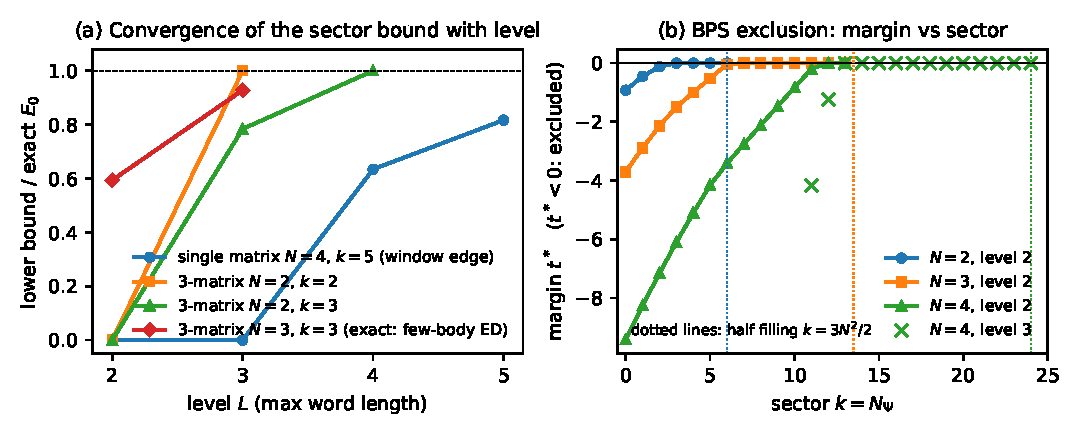
\includegraphics[width=\textwidth]{report_figs/convergence_exclusion.pdf}
\caption{(a) Sector lower bound divided by the exact ground energy (full ED at $N=2$, few-body sector ED at $N=3$) versus level for four representative sectors: each lifted sector becomes exact one level after leaving the SUSY floor. (b) BPS-exclusion margin $t^*$ versus sector: $t^*<0$ certifies that no BPS state exists in the sector at that level. At level 2 (seconds per sector) BPS states are excluded for $k\le2,6,11$ at $N=2,3,4$; level 3 adds $k=12$ at $N=4$. The BPS window sits at half filling (dotted).}
\label{fig:conv}
\end{figure}

\textbf{Beyond $N=2$ with the trace formulation.} One constraint set, evaluated at $N=2,3,4,5,10,30,100$, reproduces the analytic anchors $E_0(0)=16N^3-15N$ and $E_0(1)=16N^3-53N$ to $10^{-8}$. New results (Table~\ref{tab:largeN}): the level-2 bound is \emph{tight} for $k=2$ at every $N\ge3$ and for $k=3$ at every $N\ge4$, and equals $16N^3-(15+38k)N$; few-body ED confirms the values at $N\le5$. Together with the trivial variational state this proves
\begin{equation}
E_0(k;N)=16N^3-(15+38k)N\qquad (k\le N-1,\ \text{all cases tested}),
\end{equation}
i.e.\ the $k$-particle sector is \emph{free} for $k\le N-1$: the lowest one-particle multiplet is an $SU(N)$ adjoint, and $k$ antisymmetrised copies in the largest-Casimir component of $\wedge^k\mathbf{adj}$ are annihilated by the quartic interaction (verified explicitly at $N=3$: $\wedge^2\mathbf 8=\mathbf{10}\oplus\overline{\mathbf{10}}\oplus\mathbf 8$, with the $20$-dimensional piece free and the adjoint lifted by $+100$). The first interacting sector is $k=N$, where the bootstrap gives the first rigorous bound in an interacting sector beyond $N=2$: $E_0(3;3)\ge70.35$ at level 3 (exact $75.79$ by few-body ED in the $2925$-dimensional sector, 93\%; level 2 gives the free value $45$).

\begin{table}[t]\centering\small
\begin{tabular}{@{}lccccc@{}}\toprule
 & $N=3$ & $N=4$ & $N=5$ & $N=10$ & $N=100$\\\midrule
$E_0(2;N)$ bootstrap, level 2 (s) & 159.000 & 660.000 & 1545.000 & 15090.000 & $1.59909\times10^7$\\
$E_0(2;N)$ few-body ED & 159 & 660 & 1545 & --- & ---\\
$E_0(3;N)$ bootstrap, level 2 & $45$ (free value; exact 75.79) & 508.000 & 1355.000 & 14710.000 & ---\\
$E_0(3;N)$ few-body ED & 75.7917 & 508 & --- & --- & ---\\\bottomrule
\end{tabular}
\caption{Three-matrix model, fixed-$k$ sectors at larger $N$: rigorous lower bounds from the trace bootstrap (one constraint set, evaluated at each $N$; SCS at $N=100$) versus the few-body sector ED, which is available only where $\binom{3N^2}{k}$ is small (dashes: out of reach). All tight entries equal $16N^3-(15+38k)N$; the bootstrap values at $N=10,100$ are rigorous bounds that coincide with the formula.}
\label{tab:largeN}
\end{table}

\begin{figure}[t]\centering
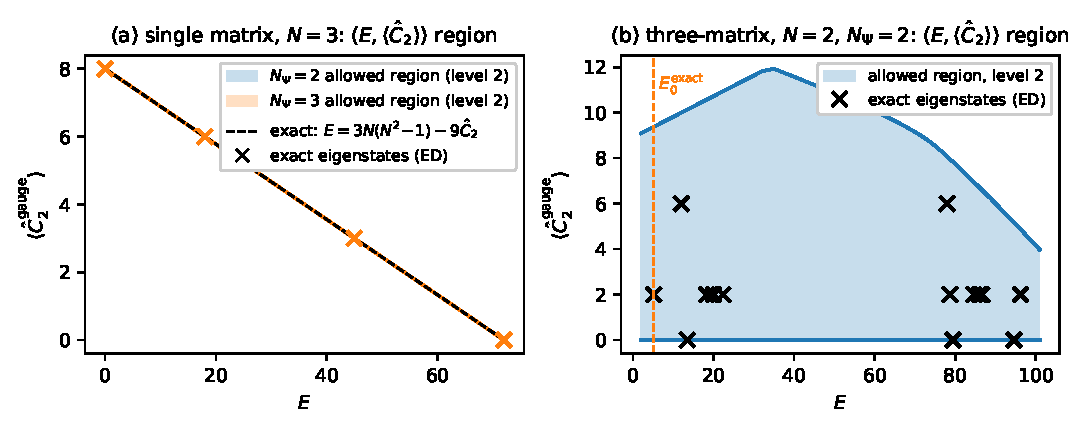
\includegraphics[width=\textwidth]{report_figs/allowed_regions.pdf}
\caption{Allowed regions in the (energy, gauge-Casimir) plane from the level-2 sector bootstrap (fix $\phi(H)=E$, extremise $\phi(\hat C_2)$), compared with the exact eigenstates (crosses). (a) Single-matrix model, $N=3$, sectors $N_\Psi=2,3$: the region has zero width and coincides with the exact line $E=3N(N^2-1)-9\hat C_2$, because the operator identity lies in the span of the constraints. (b) Three-matrix model, $N=2$, $N_\Psi=2$: a genuine two-dimensional island, rigorous and already tight at the ground-state edge.}
\label{fig:island}
\end{figure}

\textbf{Analytic refined index.} With $\mathbb Z_3$-Fourier flavour letters the Fock character $\prod_{m}\prod_{i,j}(1+t z^m u_i/u_j)$ yields, exactly, the Witten index of every complex $(c=k\bmod3,\lambda,\omega)$ --- the Euler characteristic of the strand $\mathcal H_c\to\mathcal H_{c+3}\to\cdots$ in $U(N)$ irrep $\lambda$ and flavour charge $\omega$ --- whose modulus is a lower bound on the number of BPS multiplets in the complex, with equality iff the cohomology sits in a single degree (index saturation $\Leftrightarrow$ concentration~\cite{Chang:2024fortuitySYK}). Results: at $N=2$ the index equals the ED count in all 36 complexes; the class totals are $I_c(N)=\tfrac23\,3^{3N^2/2}\cos(\tfrac{2\pi c}3+\tfrac{\pi N^2}2)$, which is \emph{exactly} the Turiaci--Witten $\cos(\pi(k-k_*)/3)$ profile about half filling ($2{:}1{:}1$ for even $N$, $0{:}1{:}1$ for odd $N$); at $N=3$ the index vanishes in every $k\equiv0$ complex; per-irrep multiplicities grow like $e^{0.75N^2}$ ($18,\,891,\,3.5\times10^5$ at $N=2,3,4$) and include gauge singlets ($6,81,1944$), whereas the single-matrix model has a single irrep per class with multiplicity $\le9$ and no singlets --- precisely the fortuitous/black-hole-like dichotomy of Chang--Lin, now quantified.

\textbf{BPS exclusion (preliminary).} Adding the linear rows $\phi(XQ)=\phi(QX)=\phi(X\bQ)=\phi(\bQ X)=0$ (satisfied by any BPS state) to \eqref{eq:sdp} and maximising a feasibility margin certifies the \emph{absence} of BPS states sector by sector. At $N=2$ this excludes $k\le2$ at level 2 and $k\le3$ at level 3 (the energy route needed one level more each time); at $N=3$ and $N=4$ level 2 already excludes $k\le6$ and $k\le11$ in seconds, level 3 adds $k=12$ at $N=4$ (Fig.~\ref{fig:conv}b). Since the index fixes the BPS count of each complex, emptying every degree but one by exclusion determines the BPS spectrum exactly.

\section{Outlook}\label{sec:outlook}
\begin{itemize}
\item \textbf{Concentration at $N=3,4$ = index $\oplus$ exclusion.} The index says the class-$0$ complexes are empty at $N=3$ and pins the counts of the others; exclusion currently empties $k\le6$ ($N=3$) and $k\le12$ ($N=4$), half-way to the window. Next: irrep-resolved exclusion (the quadratic Casimir is a trace polynomial, hence a linear row), which targets only the irreps that carry index; and exact cohomology ranks at $N=3$ ($\dim\ker Q_k-\operatorname{rank}Q_{k-3}$, sparse over a prime field) as the independent check.
\item \textbf{Near-BPS energies vs $N$.} The level-3 trace engine gives rigorous $N$-dependent bounds on the interaction energy of the first interacting sector $k=N$ in minutes per $N$; with few-body ED at $N=4$ ($k=4$, dim $1.9\times10^5$, Lanczos) as calibration this is a direct test of the super-Schwarzian scaling.
\item \textbf{Sparse ED / Lanczos at $N=3$} for the window sectors (dimensions to $2\times10^7$; feasible with a matrix-free implementation) --- energies, exact BPS counts, and the Turiaci--Witten chaos test on the singular values of $Q_k$ (Q2).
\item \textbf{Analytic.} A proof of the free-sector formula (a short Casimir argument); large-$N$ asymptotics of the per-irrep index (saddle point of the character integral); the traceless $su(N)$ variant and $p=2$ models (Q3).
\item \textbf{Solvers.} Level 4 is assembled but not solved to tolerance (Appendix); the dual (SDPA/SDPB) form after exact elimination, or the reversal $\mathbb Z_2$ that halves every cone, would make it interior-point feasible.
\end{itemize}

\appendix
\section{Numerical implementation}
\begin{itemize}
\item \textbf{Finite-$N$ engine} (\texttt{sector\_bootstrap.py}): open words are built as rectangular sector-to-sector blocks (the $2^{pN^2}$ space is never formed); an isotypic reducer (highest weights + $J_-$ lowering, fermionic-sign-correct $\mathbb Z_3$ Fock unitary) maps every operator to its $D=\sum_Rm_R^2$ invariant components the moment it is built; touched and EOM spans are accumulated as streaming $2D\times2D$ Gram matrices; each cone is rescaled by a diagonal congruence. A diagnostic evaluates every constraint on the exact multiplet-averaged ground state and caught a round-off Hermitian part being normalised into a spurious constraint (the cutoff must be relative to $\|X\|$).
\item \textbf{Trace algebra} (\texttt{trace\_algebra.py}): a single primitive --- the adjacent swap of a \emph{routed term} (letters in operator order plus a routing permutation; the anticommutator branch rewires the routing by union--find, closed loops give factors of $N$) --- from which canonical cyclic forms, trace-factor ordering, products, daggers, $[H,\cdot]$, self-symmetry reductions ($\Tr[\ell\ell]=0$, $TT=\tfrac12\{T,T\}$) and finite-$N$ antisymmetriser relations all follow. Coefficients are polynomials in $N$. Every identity is verified against explicit operators at $N=2,3$ (1000 random routed terms to $10^{-15}$; $\{Q,\bQ\}=H$ recovered by the algebra itself).
\item \textbf{Assembly and conditioning} (\texttt{trace\_bootstrap.py}): variables generated by closure; reality imposed at the variable level (halves the unknowns); unit-norm rows; 't~Hooft column scaling $\phi(m)\to N^{\sum(1+L_i/2)}$ and objective $/N^3$ (needed beyond $N\approx30$); pivoted-QR pruning of redundant equality rows for Clarabel; direct Clarabel/SCS interfaces (no modelling layer). Solver settings that matter: Clarabel with chordal decomposition off and equilibration on; SCS with $\rho_x=10^{-3}$, Apple-Accelerate LDL, fixed scaling. Fixed-$N$ parallel build (8 forked workers) produces the level-4 problem (51k monomials, cones to 168) in 25~s.
\item \textbf{Cost and limits.} Levels 2--3 cost seconds to minutes at any $N$ and $\le5$~GB. Level 4 is solver-limited: interior-point codes carry a dense $n_{\rm svec}^2$ block per PSD cone ($\sim25$~GB for a 168-dimensional complex cone), and SCS reaches only $10^{-2}$ residuals in 6000 iterations. Every run is preceded by a memory estimate and guarded by a watchdog (budget 10~GB).
\item \textbf{Few-body ED and index} (\texttt{fewbody.py}, \texttt{bps\_index.py}): $k$-subset bases with operators applied by explicit index sums; index by exact integer arithmetic (the Fock generating function as integer shifts on the $SU(N)$ torus, Weyl alternating sum for irrep multiplicities), seconds for $N\le4$.
\end{itemize}

\begin{thebibliography}{9}\small\setlength{\itemsep}{0pt}
\bibitem{Chen:2025fortuity} Y.~Chen, \emph{Fortuity with a Single Matrix}, arXiv:2511.00790.
\bibitem{Chang:2024fortuitySYK} C.-M.~Chang, Y.~Chen, B.~S.~Sia, Z.~Yang, \emph{Fortuity in SYK models}, arXiv:2412.06902.
\bibitem{Chang:2024covering} C.-M.~Chang, Y.-H.~Lin, \emph{Holographic covering and the fortuity of black holes}, arXiv:2402.10129.
\bibitem{Turiaci:2023N2JT} G.~J.~Turiaci, E.~Witten, \emph{$\mathcal N=2$ JT supergravity and matrix models}, arXiv:2305.19438.
\bibitem{Fu:2016SUSYSYK} W.~Fu, D.~Gaiotto, J.~Maldacena, S.~Sachdev, \emph{Supersymmetric SYK models}, arXiv:1610.08917.
\bibitem{Han:2020bootstrapMQM} X.~Han, S.~A.~Hartnoll, J.~Kruthoff, \emph{Bootstrapping matrix quantum mechanics}, arXiv:2004.10212.
\bibitem{Lin:2025highprecision} H.~W.~Lin, Z.~Zheng, \emph{High-precision bootstrap of multimatrix quantum mechanics}, arXiv:2507.21007.
\bibitem{Cho:2024thermal} M.~Cho, B.~Gabai, J.~Sandor, X.~Yin, \emph{Thermal bootstrap of matrix quantum mechanics}, arXiv:2410.04262.
\bibitem{Laliberte:2025SUSYbootstrap} S.~Laliberte, B.~McPeak, \emph{Bootstrapping supersymmetric (matrix) quantum mechanics}, arXiv:2510.01356.
\end{thebibliography}
\end{document}
